%%%%%%%% Sample LaTeX input for Complex Systems %%%%%%%%%%% 
% Revision 4, Jun 27, 2018
%
% This is a LaTeX input file  
% Text following % on a particular line is treated as a comment, and 
% ignored by LaTeX.  
% You do not need to type any text that follows a % 
% 
\documentclass{article}

\usepackage{graphicx,hyperref}
\usepackage{amssymb,ComplexSystems}
\usepackage{tikz}
\usepackage{scalefnt}

\usetikzlibrary{automata, positioning, arrows}
\usepackage{underscore}
\graphicspath{ {./images/} }

% complex-systems.sty is the macro package for Complex Systems.
% It is available at
% http://www.complex-systems.com/samples/complex-systems.sty
% epsf.sty is the preferred graphics import method
\makeindex

\begin{document}

\title{Documentation - Data Bases 2%
% Use \\ to indicate line breaks in titles longer than about 
% 55 characters. 
%
}

\author{\authname{Marco Fasanella}\\[2pt] 
% Use \\[2pt] to end the line and add space between author name and affiliation. 
\authadd{MsC Computer Science, Polimi}\\
\authadd{C.P. 10617541}\\
\and
% For extra space, precede the second set of authors with \and.
\authname{Nicola Dean}\\
\authadd{MsC Computer Science, Polimi}\\
\authadd{C.P. 106-----}\\
% Do not use a ``.'' at the end of any line in the address. 
}

% The following specifies the running headings 
%
% Each running heading should be less than about 50 characters long. 
% If necessary, give a shortened version of the title. 
%
% Use initials for first and second names. If all author names do not fit, truncate the 
% list and end with ``et al.''.
\markboth{Data Base 2 Project} 
{Design Documentation}

\maketitle
% End title section

\begin{abstract}
This document describes design 
\end{abstract}

% The text of the paper follows. All of the text should be in the same file. 
% Use separate files for large tabular material and graphics.
%\printindex
\section{Introduction}
\label{intro}
% \label is a hyperlink target for cross-referencing to this section using \ref{intro} (optional).
Il circuito descritto si occupa di leggere e rielaborare i dati da RAM producendo un'immagine con nitidezza più alta e quindi più leggibile. 


Nel circuito è stato scelto di dividere in 3 la computazione con moduli in cascata.
\subsection{Specifica}
 \begin{figure}[h]
\centering
\caption{Interfaccia del Componente)}
\end{figure}
I segnali da considerare sono i seguenti:
\newline
\section{Triggers}
\subsection{Insolvent Users}
\begin{verbatim}
create trigger INSOLVENT_USER
    after insert on Orders
    for each row
begin
    if ( new.status = false) then
    update Users set Users.insolvent = true where Users.id = new.userId;
    insert into FailedPayments (userId,orderId,faildate) 
    values (new.userId,new.id,CURRENT_TIMESTAMP);
end if;
\end{verbatim}



\begin{verbatim}
create trigger INSOLVENT_USER_REMOVAL
    after update on Orders
    for each row
begin
    if (new.status = true) AND -- user payed a suspended order i check if all his pending order are payed (if yes remove flag)
			(select count(*) from Orders as o where o.userId=new.userId and o.status = false) = 0
		then
    update Users set Users.insolvent = false where Users.id = new.userId;
end if;
if (new.status = false AND old.status = new.status)  then
			insert into FailedPayments (userId,orderId,faildate) values (new.userId,new.id,CURRENT_TIMESTAMP);
end if;
\end{verbatim}

\begin{verbatim}

\end{verbatim}

\begin{verbatim}

\end{verbatim}


\section{SQL Description}
\section{Extra hypotesis}
\section{ER Diagram}

\begin{figure}[hbt!]
\centering
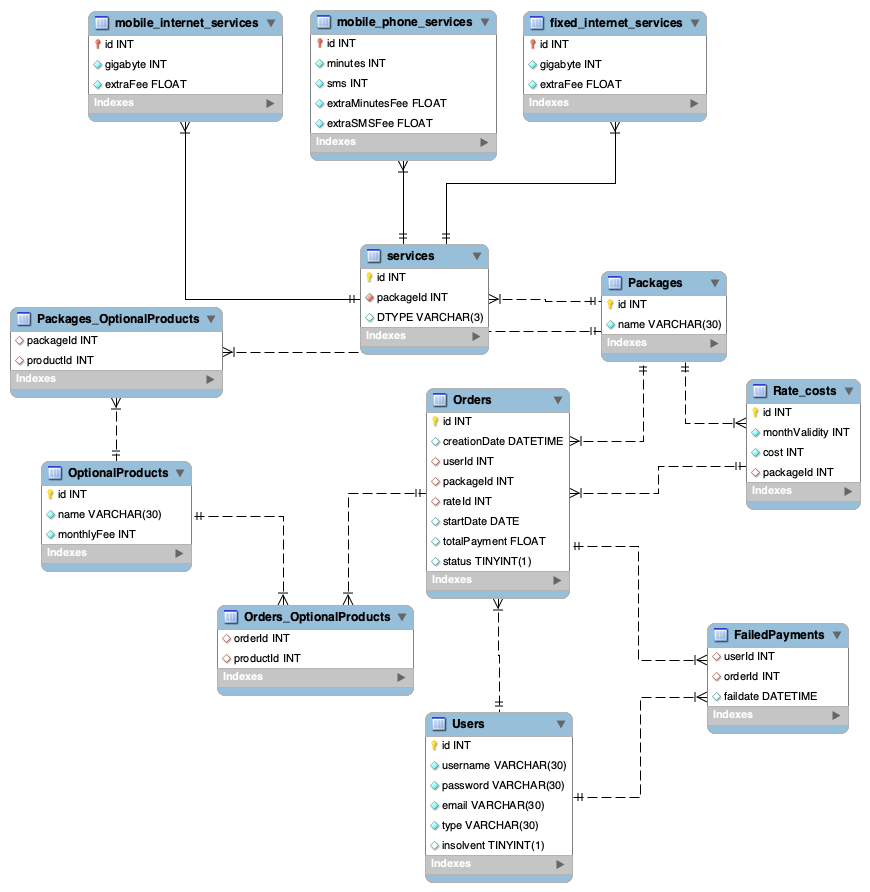
\includegraphics[width=0.86\textwidth]{er.png}
\caption{ER Diagram}
\end{figure}


\section{Relation Model}
\section{ORM Description}
\section{Application Components}
\section{UML sequence diagrams}

\end{document}